\chapter{Моделирование}

\section{Концептуальная модель}

\textbf{Система анализа тепловых утечек} --- программный комплекс, выполняющий следующие основные функции:

\begin{itemize}
		\item Оценка энергетической эффективности зданий городской застройки;
		\item Выдача результатов оценивания по запросу;
		\item Обработка ИК снимков;
		\item Упрощение процесса проведения ИК съёмки пользователями.
\end{itemize}

\textbf{Пути реализации основных функций:}

\begin{itemize}
	\item Обнаружение критичных областей и вычисления средних значений показателей распределения тепла по ИК снимкам;
	\item Предоставление веб-доступа к результатам обследования;
	\item Геометрическая коррекция изображений и учета внешних условий съёмки;
	\item Программное обеспечение процесса проведения ИК съемки.
\end{itemize}
 
\textbf{Структурная основа реализации:}

\begin{itemize}
	\item Методы статистического анализа;
	\item Способы визуализации данных;
	\item Алгоритмы нормализации ИК снимков по инвариантным признакам спутниковых снимков;
	\item Клиент-серверная архитектура.
\end{itemize}

\textbf{Направленность функционирования системы}: обеспечение информационной поддержки процесса обнаружения, обследования, контроля и устранения тепловых утечек.
 
\textbf{Цель функционирования системы}: повышение качества обследования жилых объектов на предмет тепловой энергоэффективности. \\
 
\textbf{Программный интерфейс (API)} для системы анализа тепловых утечек городской застройки.

\begin{enumerate}
 
	\item \textbf{Основные функции}:

	\begin{enumerate}[label=\labelenumi.\arabic*]
		\item Сбор данных; \label{cm:f:1}
		\item Унификация данных, поступающих в систему анализа; \label{cm:f:2}
		\item Обеспечение их корректности; \label{cm:f:3}
		\item Обеспечение доступности данных для системы анализа; \label{cm:f:4}
		\item Предоставление результатов анализа клиентским приложениям. \label{cm:f:5}
	\end{enumerate}

	\item \textbf{Пути реализации основных функций}:

	\begin{enumerate}
		\item Приём пакетов данных от различных источников;
		\item Преобразование данных в одинаковый формат;
		\item Проверка пакетов входных данных на соответствие требованиям;
		\item Взаимодействие с БД системы анализа;
		\item Обработка внешних запросов на результаты анализа утечек.
	\end{enumerate}

	\item \textbf{Структурная основа реализации}:

	\begin{enumerate}
		\item Для функций \ref{cm:f:1}, \ref{cm:f:5}: сетевые протоколы обмена информацией;
		\item Для функции \ref{cm:f:2}: требования системы анализа тепловых утечек;
		\item Для функции \ref{cm:f:3}: методы фильтрации нежелательного контента;
		\item Для функции \ref{cm:f:4}: централизованный подход к управлению данными в СУБД.
	\end{enumerate}

	\item \textbf{Направленность функционирования системы}: расширение географической области, охватываемой системой анализа и увеличение числа пользователей системы анализа.

	\item \textbf{Цели функционирования системы}: предоставление набора функций, реализуемых системой анализа тепловых утечек, сторонним программам вне зависимости от их платформы и аппаратного обеспечения.

\end{enumerate}

\section{Системно-структурная модель}

\par 
	На рисунке \ref{ssm:0} изображена системно-структурная модель системы анализа тепловых утечек. Внедрение в неё новых структурных элементов -- программного интерфейса и мобильного приложения -- приводит к изменению состава таких подсистем, как веб-приложение и модуля работы с ИК изображениями. Модели этих подсистем представлены на рисунках [\ref{ssm:1}, \ref{ssm:3}] соответственно.

	 \begin{figure}[h!]
      \centering
      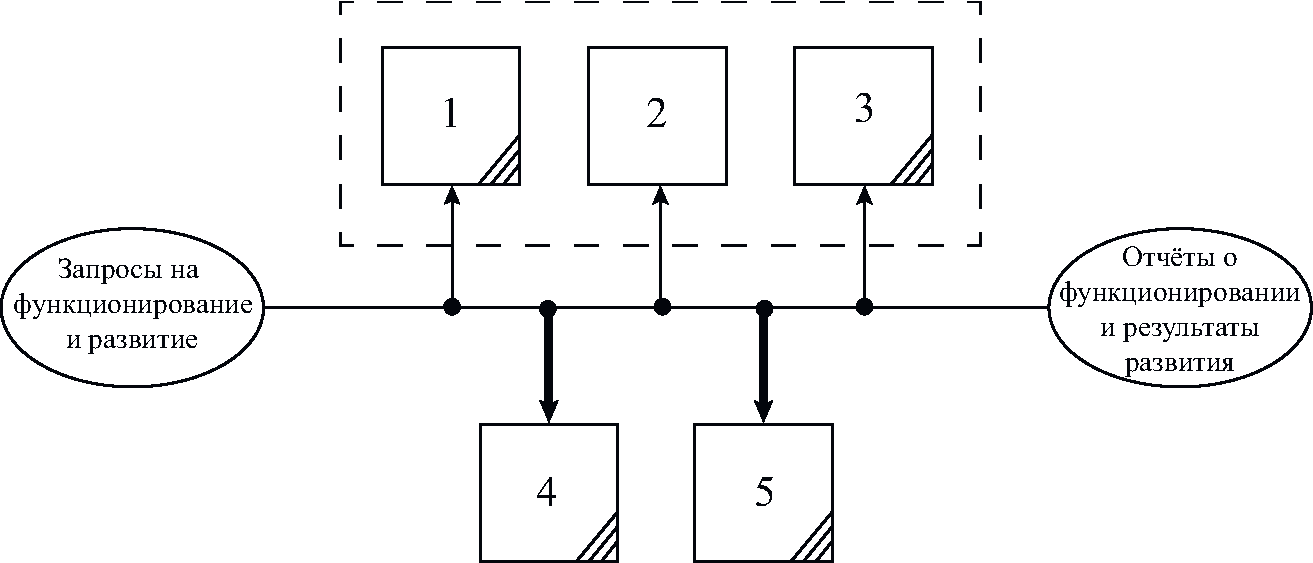
\includegraphics[width=0.9\textwidth]{images/ssm/0}
      \caption{Системно-структурная модель системы анализа тепловых утечек: 1 - веб-приложение, 2 - подсистема управления данными, 3 - модуль работы с ИК изображениями, 4 - мобильное приложение, 5 - программный интерфейс (API)}
      \label{ssm:0}
    \end{figure}

\pagebreak

\par 
	Структурные компоненты web-приложения представлены разделами, с которыми работают его пользователи (рисунок \ref{ssm:1}). Работа каждого раздела обеспечивается web-сервером и множеством программных сценариев, генерирующих динамические web-страницы, содержащие информацию, соответствующую названию раздела.

	\begin{figure}[t!]
      \centering
      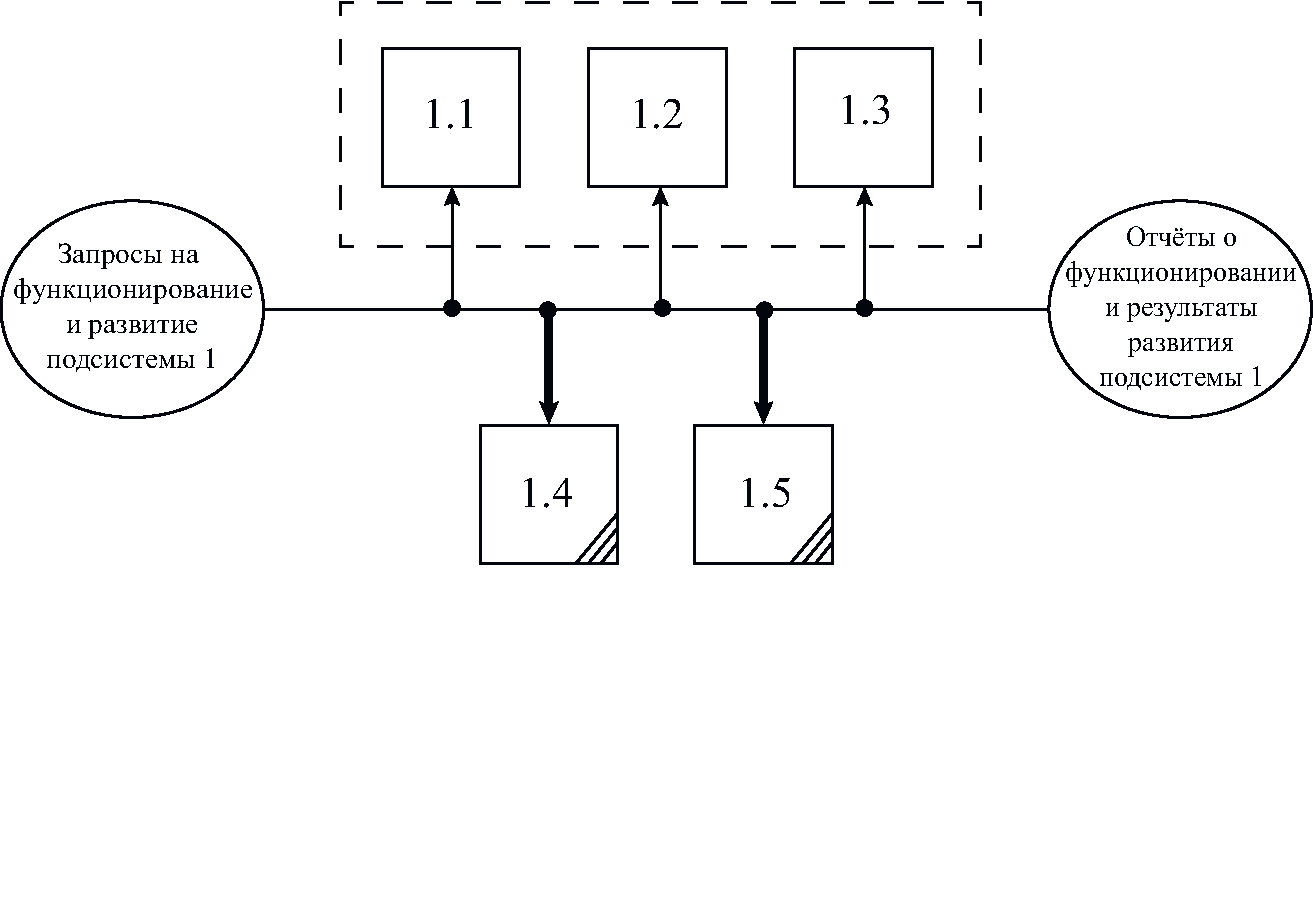
\includegraphics[width=0.9\textwidth]{images/ssm/1}
      \caption{Системно-структурная модель веб-приложения: 1.1 - блок отображения карты, 1.2 - блок отображения оценок энергоэффективности и энергозатрат, 1.3 - блок представления изображений, 1.4 - раздел «личного кабинета», 1.5 - раздел загрузки пользовательских данных}
      \label{ssm:1}
    \end{figure}

\par
	Компоненты модуля работы с ИК изображениями (рисунок \ref{ssm:3}) разделены по характеру выполняемых преобразований: подсистема 3.1 решает задачу распознавания зданий с ИК аэроснимков, описанную в [***MyHEAT***], процедуры обработки в подсистеме 3.2 устраняют отклонения, вызванные локальными изменениями климата, на снимках, подсистема 3.3 использует алгоритмы математической статистики для итоговых расчётов.

\pagebreak

	В связи с тем, что в систему анализа тепловых утечек внедряется новый вид съёмки, очевидно, что некоторые подсистемы претерпят изменения, которые отражены в алгоритмических моделях. Подсистемы 3.1 и 3.2 являются исключениями, поскольку для наземной съёмки отдельных зданий они не актуальны. Многие задачи обработки наземных снимков берут на себя программные клиенты - мобильные приложения.

	\begin{figure}[t!]
      \centering
      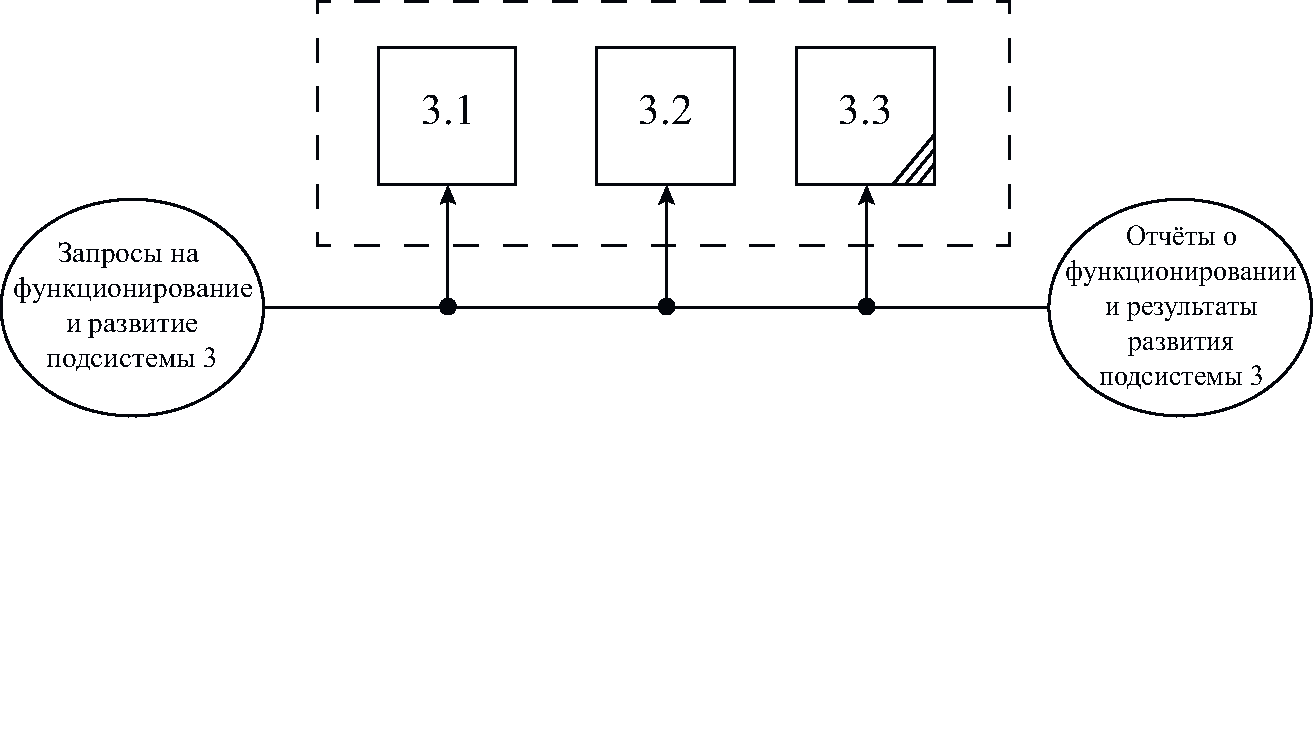
\includegraphics[width=0.9\textwidth]{images/ssm/3}
      \caption{Системно-структурная модель модуля работы с ИК изображениями: 3.1 - подсистема фотограмметрической обработки ИК снимков, 3.2 - подсистема коррекции по микроклиматическим условиям, 3.3 - подсистема расчёта оценки энергоэффективности}
      \label{ssm:3}
    \end{figure}

\par
	В модели программного интерфейса (API) системы анализа тепловых утечек, представленной на рисунке \ref{ssm:5}, в качестве подсистем прототипа были взяты стандартные компоненты, участвующие в работе большинства API относительно крупных программных комплексов. 
	
	В рамках системы анализа тепловых утечек специфика API заключается в наличии подсистемы 5.5. Это связано с характерными особенностями данных, поступающих в систему. Например, в систему могут поступать данные с ИК камер различных производителей, и, кроме того, данные различных типов съёмки. Расширение спектра возможных источников данных - одна из причин внедрения API в основную систему.

\pagebreak

	\begin{figure}[t!]
      \centering
      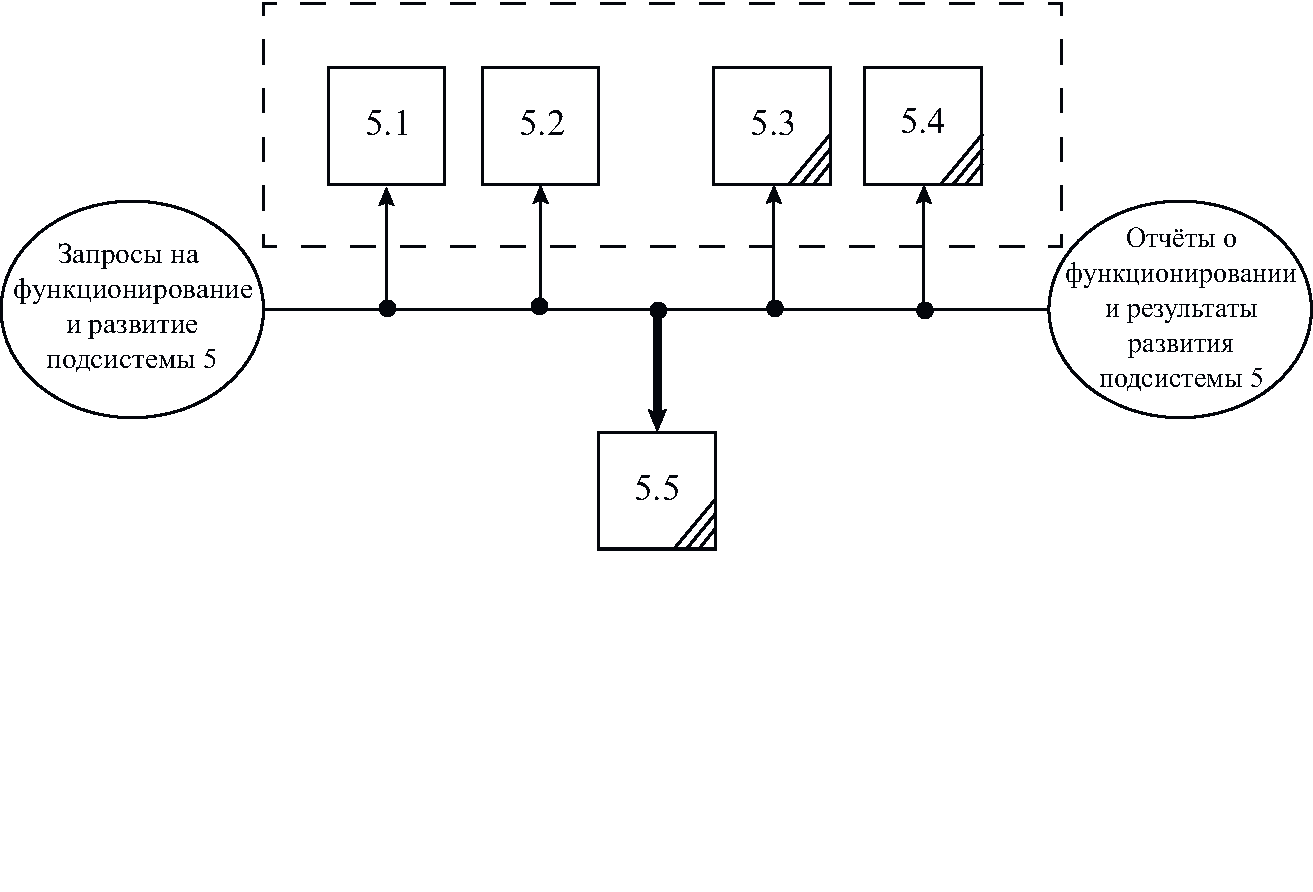
\includegraphics[width=0.9\textwidth]{images/ssm/5}
      \caption{Системно-структурная модель программного интерфейса: 5.1 - подсистема приёма запросов и отправки данных,  5.2 - подсистема аутентификации пользователей, 5.3 - подсистема формирования запросов к БД, 5.4 - подсистема валидации данных, 5.5 - подсистема унификации и форматирования данных}
      \label{ssm:5}
    \end{figure}

\section{Функционально-структурная модель}

\par
	Все функции, выполняемые системами анализа тепловых утечек, можно объединить в один функциональный блок “Оценить энергетическую эффективность зданий”, как показано на диаграмме, изображенной на рисунке \ref{fsm:0}. Рассмотрение функциональной структуры системы в целом важно при моделировании разрабатываемого программного интерфейса, поскольку это даёт представление о взаимосвязи информационных потоков между смежными функциями всей системы, а также с её внешней средой. Модели выполнены в соответствии с нотацией \texttt{IDEF0}.

	\begin{figure}[t!]
      \centering
      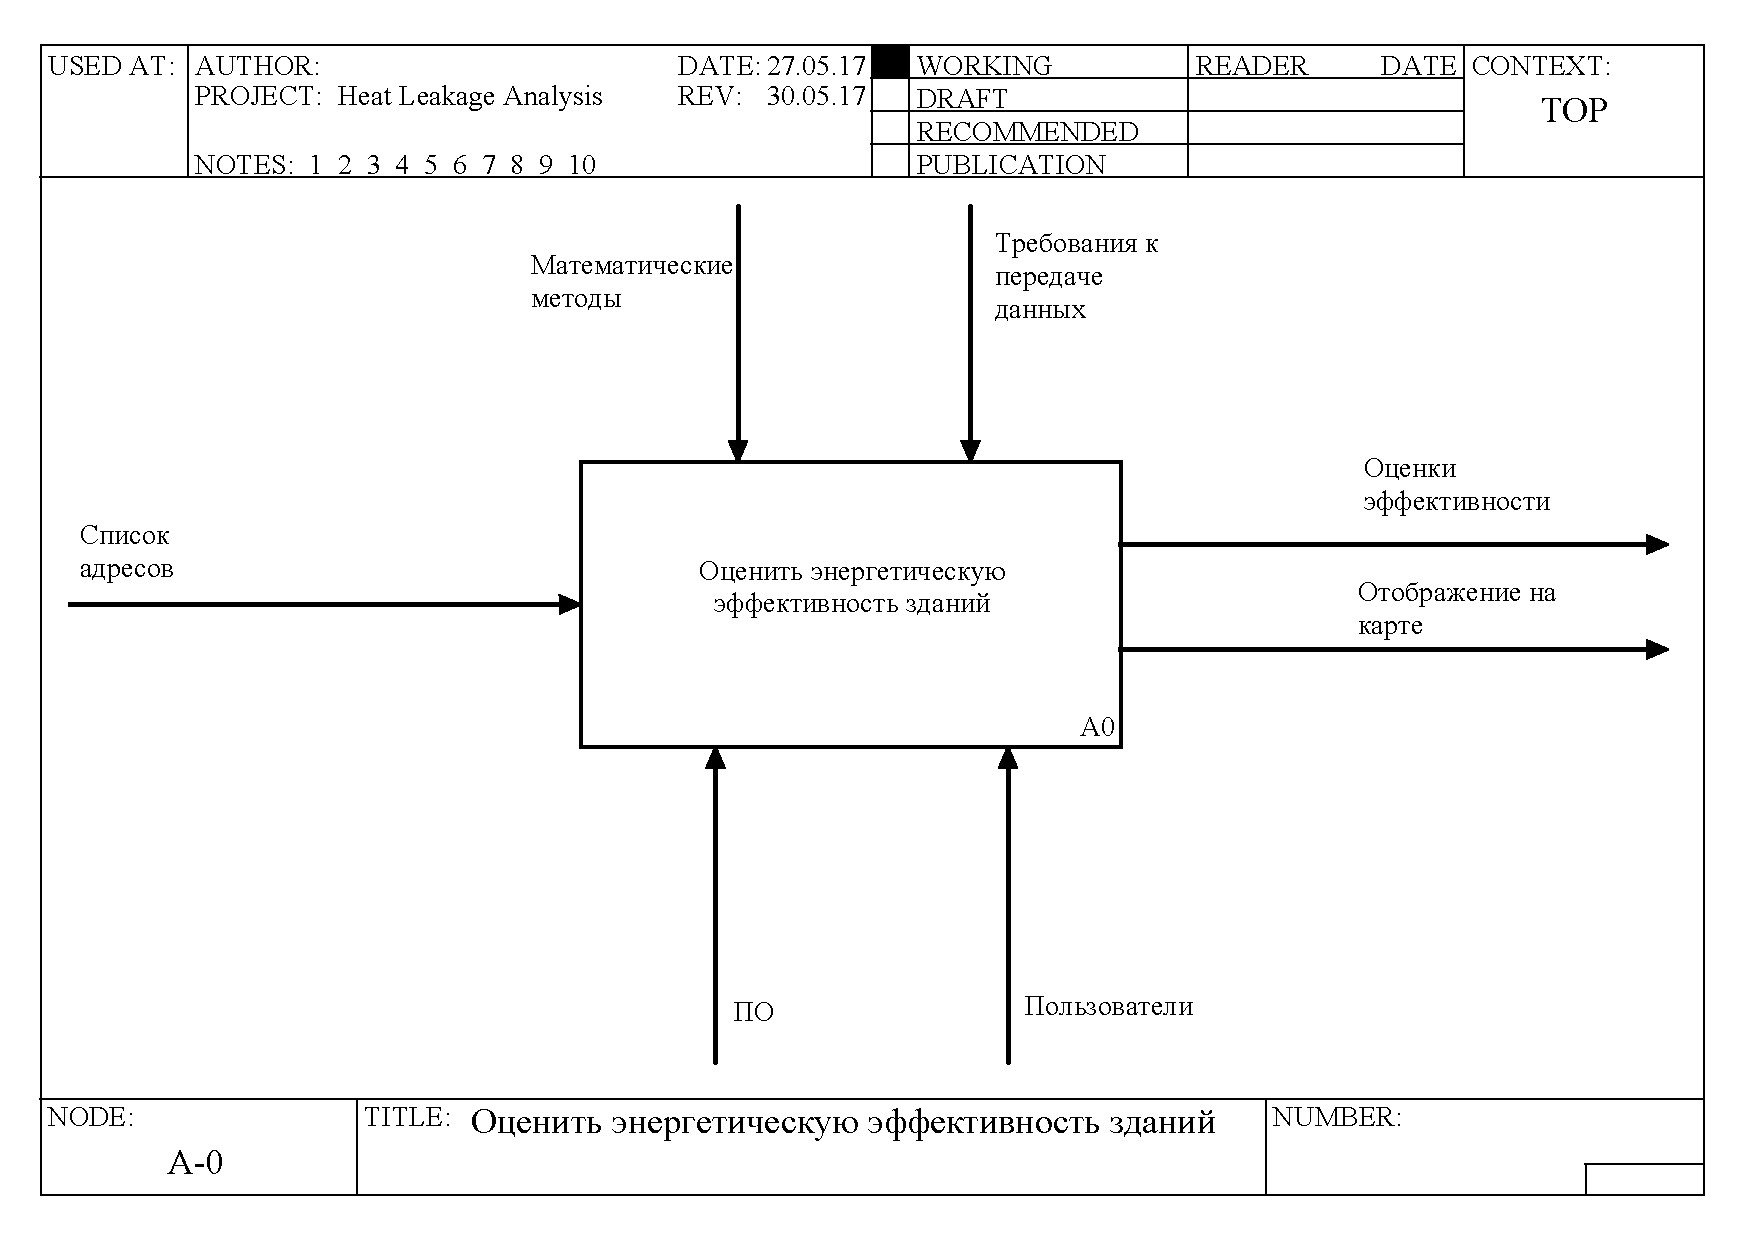
\includegraphics[width=0.9\textwidth]{images/fsm/0}
      \caption{Контекстная диаграмма функционально-структурной модели предлагаемого решения}
      \label{fsm:0}
    \end{figure}

\par
    Диаграмма декомпозиции 1 уровня включает в себя набор основных функций, которые выполняются подсистемами, перечисленными в системно-структурной модели \ref{fsm:1}. Так, функциональный блок A3 выполняется программным интерфейсом (подсистема 5, рисунок \ref{ssm:5}). Некоторые подсистемы могут участвовать в работе нескольких функций. Например, за работу блоков A2 и A6 отвечает мобильное приложение (подсистема 3, рисунок \ref{ssm:3}).

	Описание математических алгоритмов содержится в некоторых алгоритмических моделях, приведённых в разделе \ref{sec:models:algo}. Под клиентскими приложениями понимается ПО, которое отображает карты энергоэффективности зданий (в частности, мобильное и web-приложения).

	\begin{figure}[t!]
      \centering
      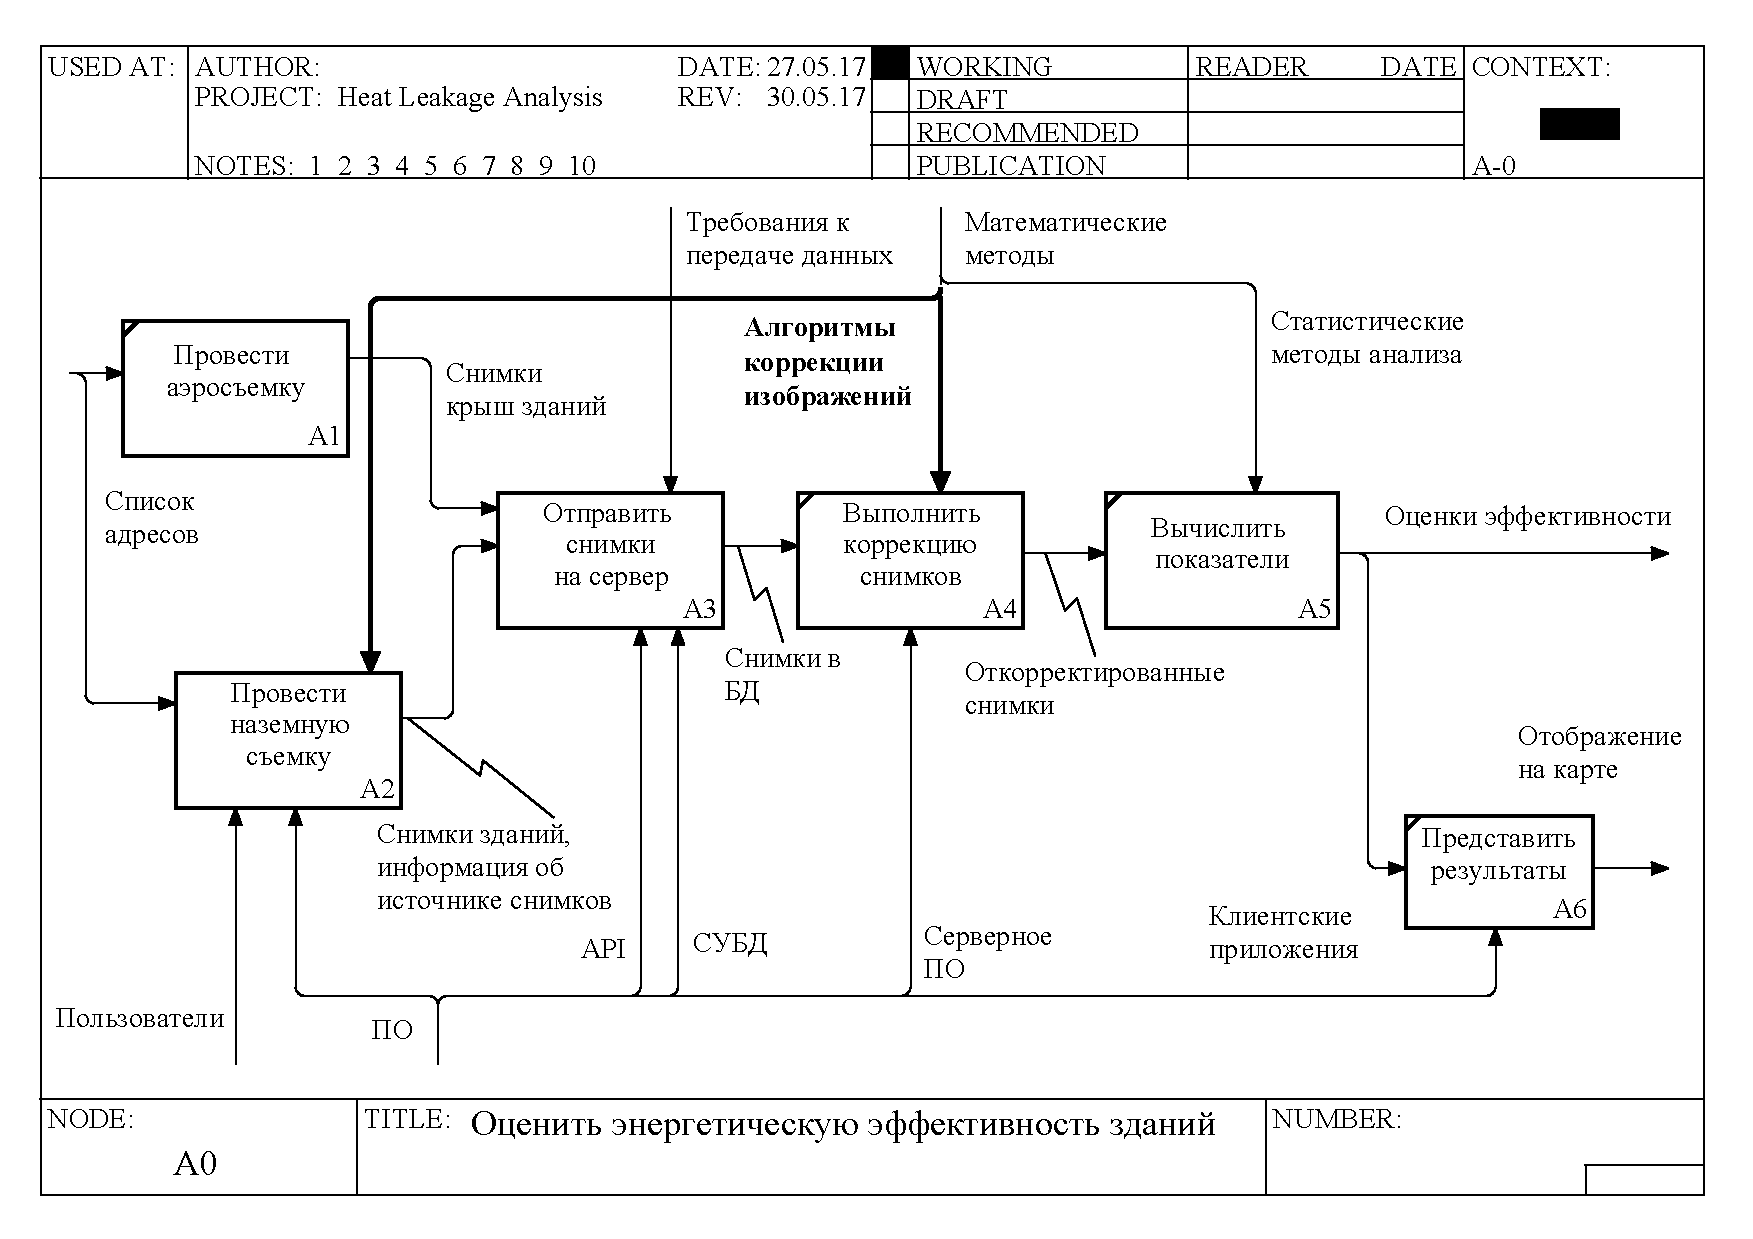
\includegraphics[width=0.7\textwidth]{images/fsm/1}
      \caption{Диаграмма декомпозиции 1 уровня функционально-структурной модели предлагаемого решения}
      \label{fsm:1}
    \end{figure}

\par
    На рисунке \ref{fsm:2} представлена диаграмма декомпозиции блока \textit{“Отправить снимки на сервер”}. Все функциональные блоки в этой диаграмме задействуют API, поэтому она представляет наибольший интерес среди остальных блоков узла A0.

    \begin{figure}[h!]
      \centering
      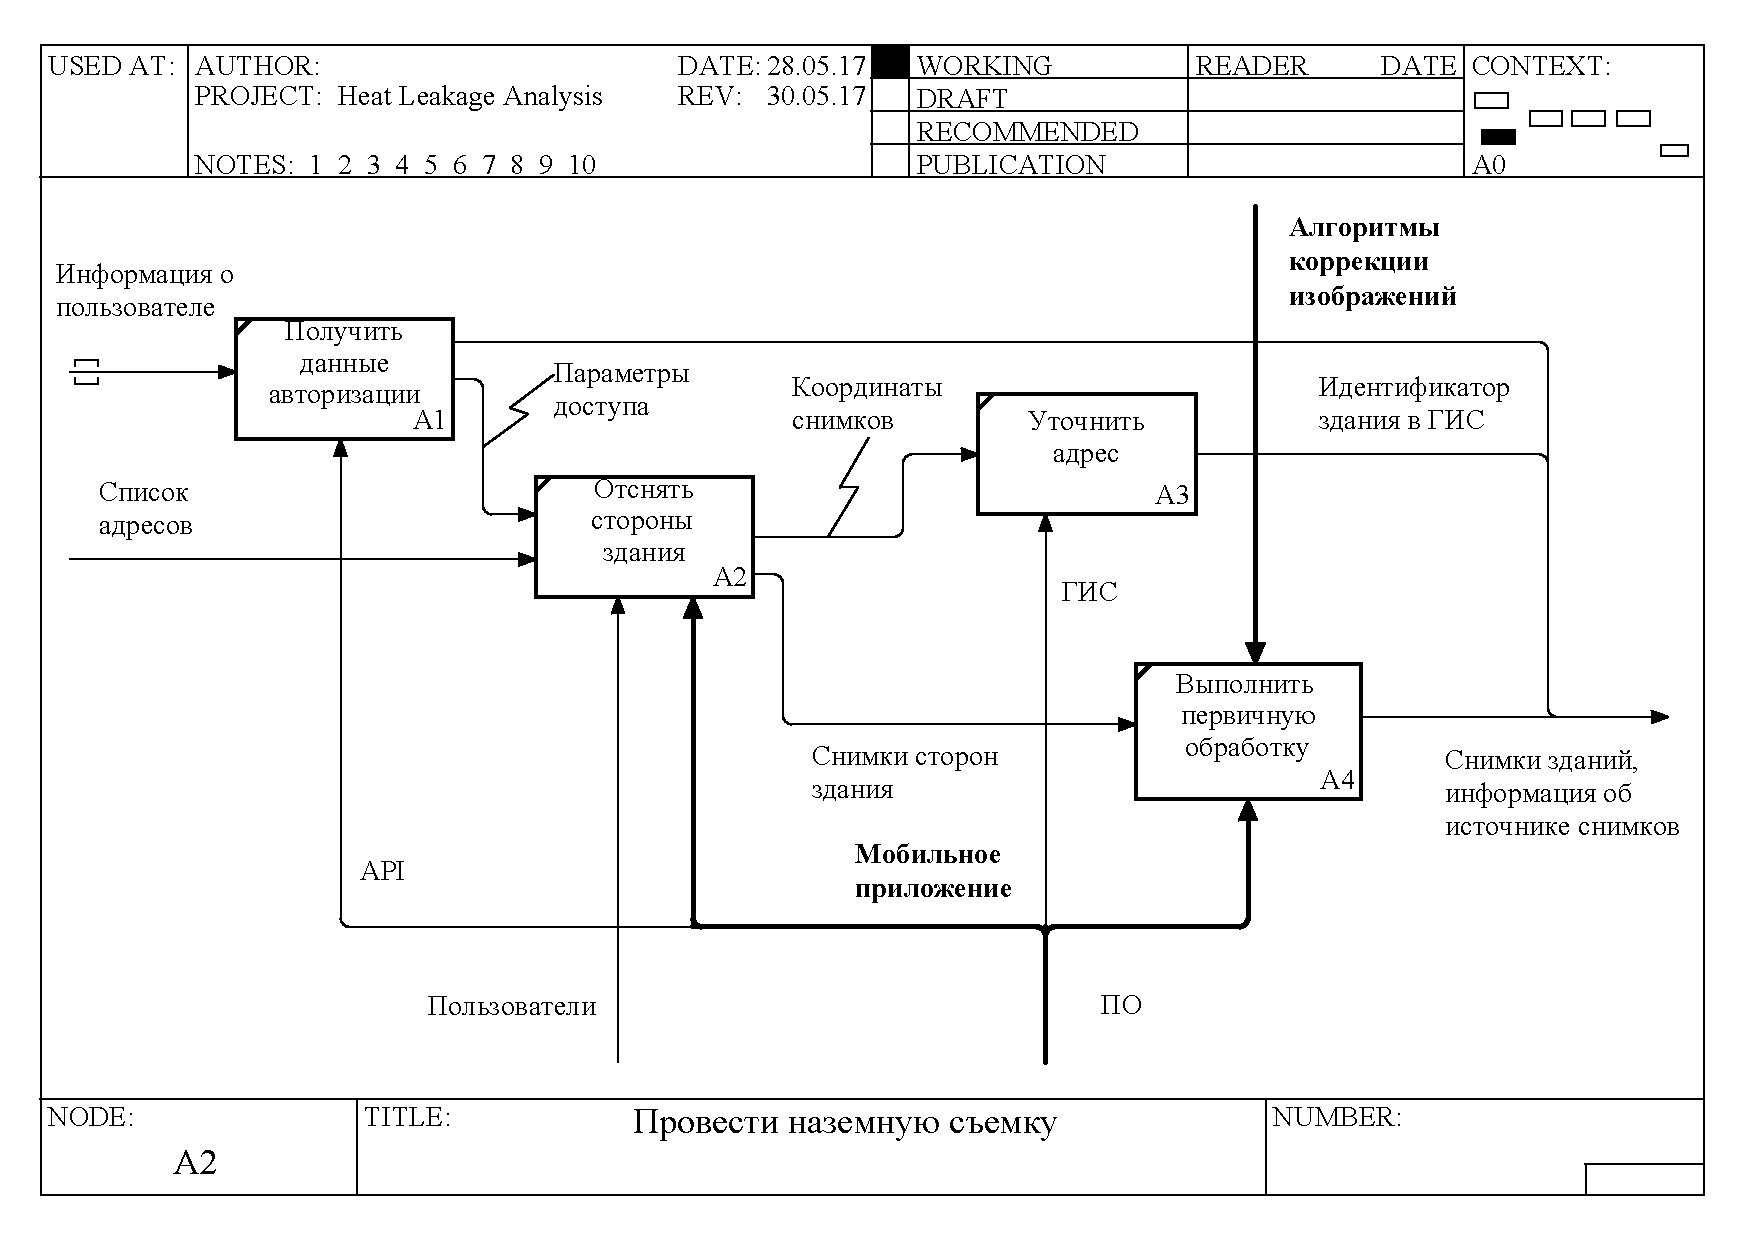
\includegraphics[width=0.7\textwidth]{images/fsm/2}
      \caption{Диаграмма декомпозиции блока A3 функционально-структурной модели предлагаемого решения}
      \label{fsm:2}
    \end{figure}

\pagebreak

\section{Алгоритмическая модель}
\label{sec:models:algo}
	
\par
	В разделе \ref{sec:models:algo:before} приведены алгоритмы процессов работы системы до внедрения в неё новых подсистем. В разделе \ref{sec:models:algo:after} представлены алгоритмы, в которых происходят наиболее существенные изменения после внедрения внедряемых подсистем, а также алгоритм работы разрабатываемого программного интерфейса.

\subsection{Алгоритмическая модель прототипа}
\label{sec:models:algo:before}

	\begin{figure}[h!]
      \centering
      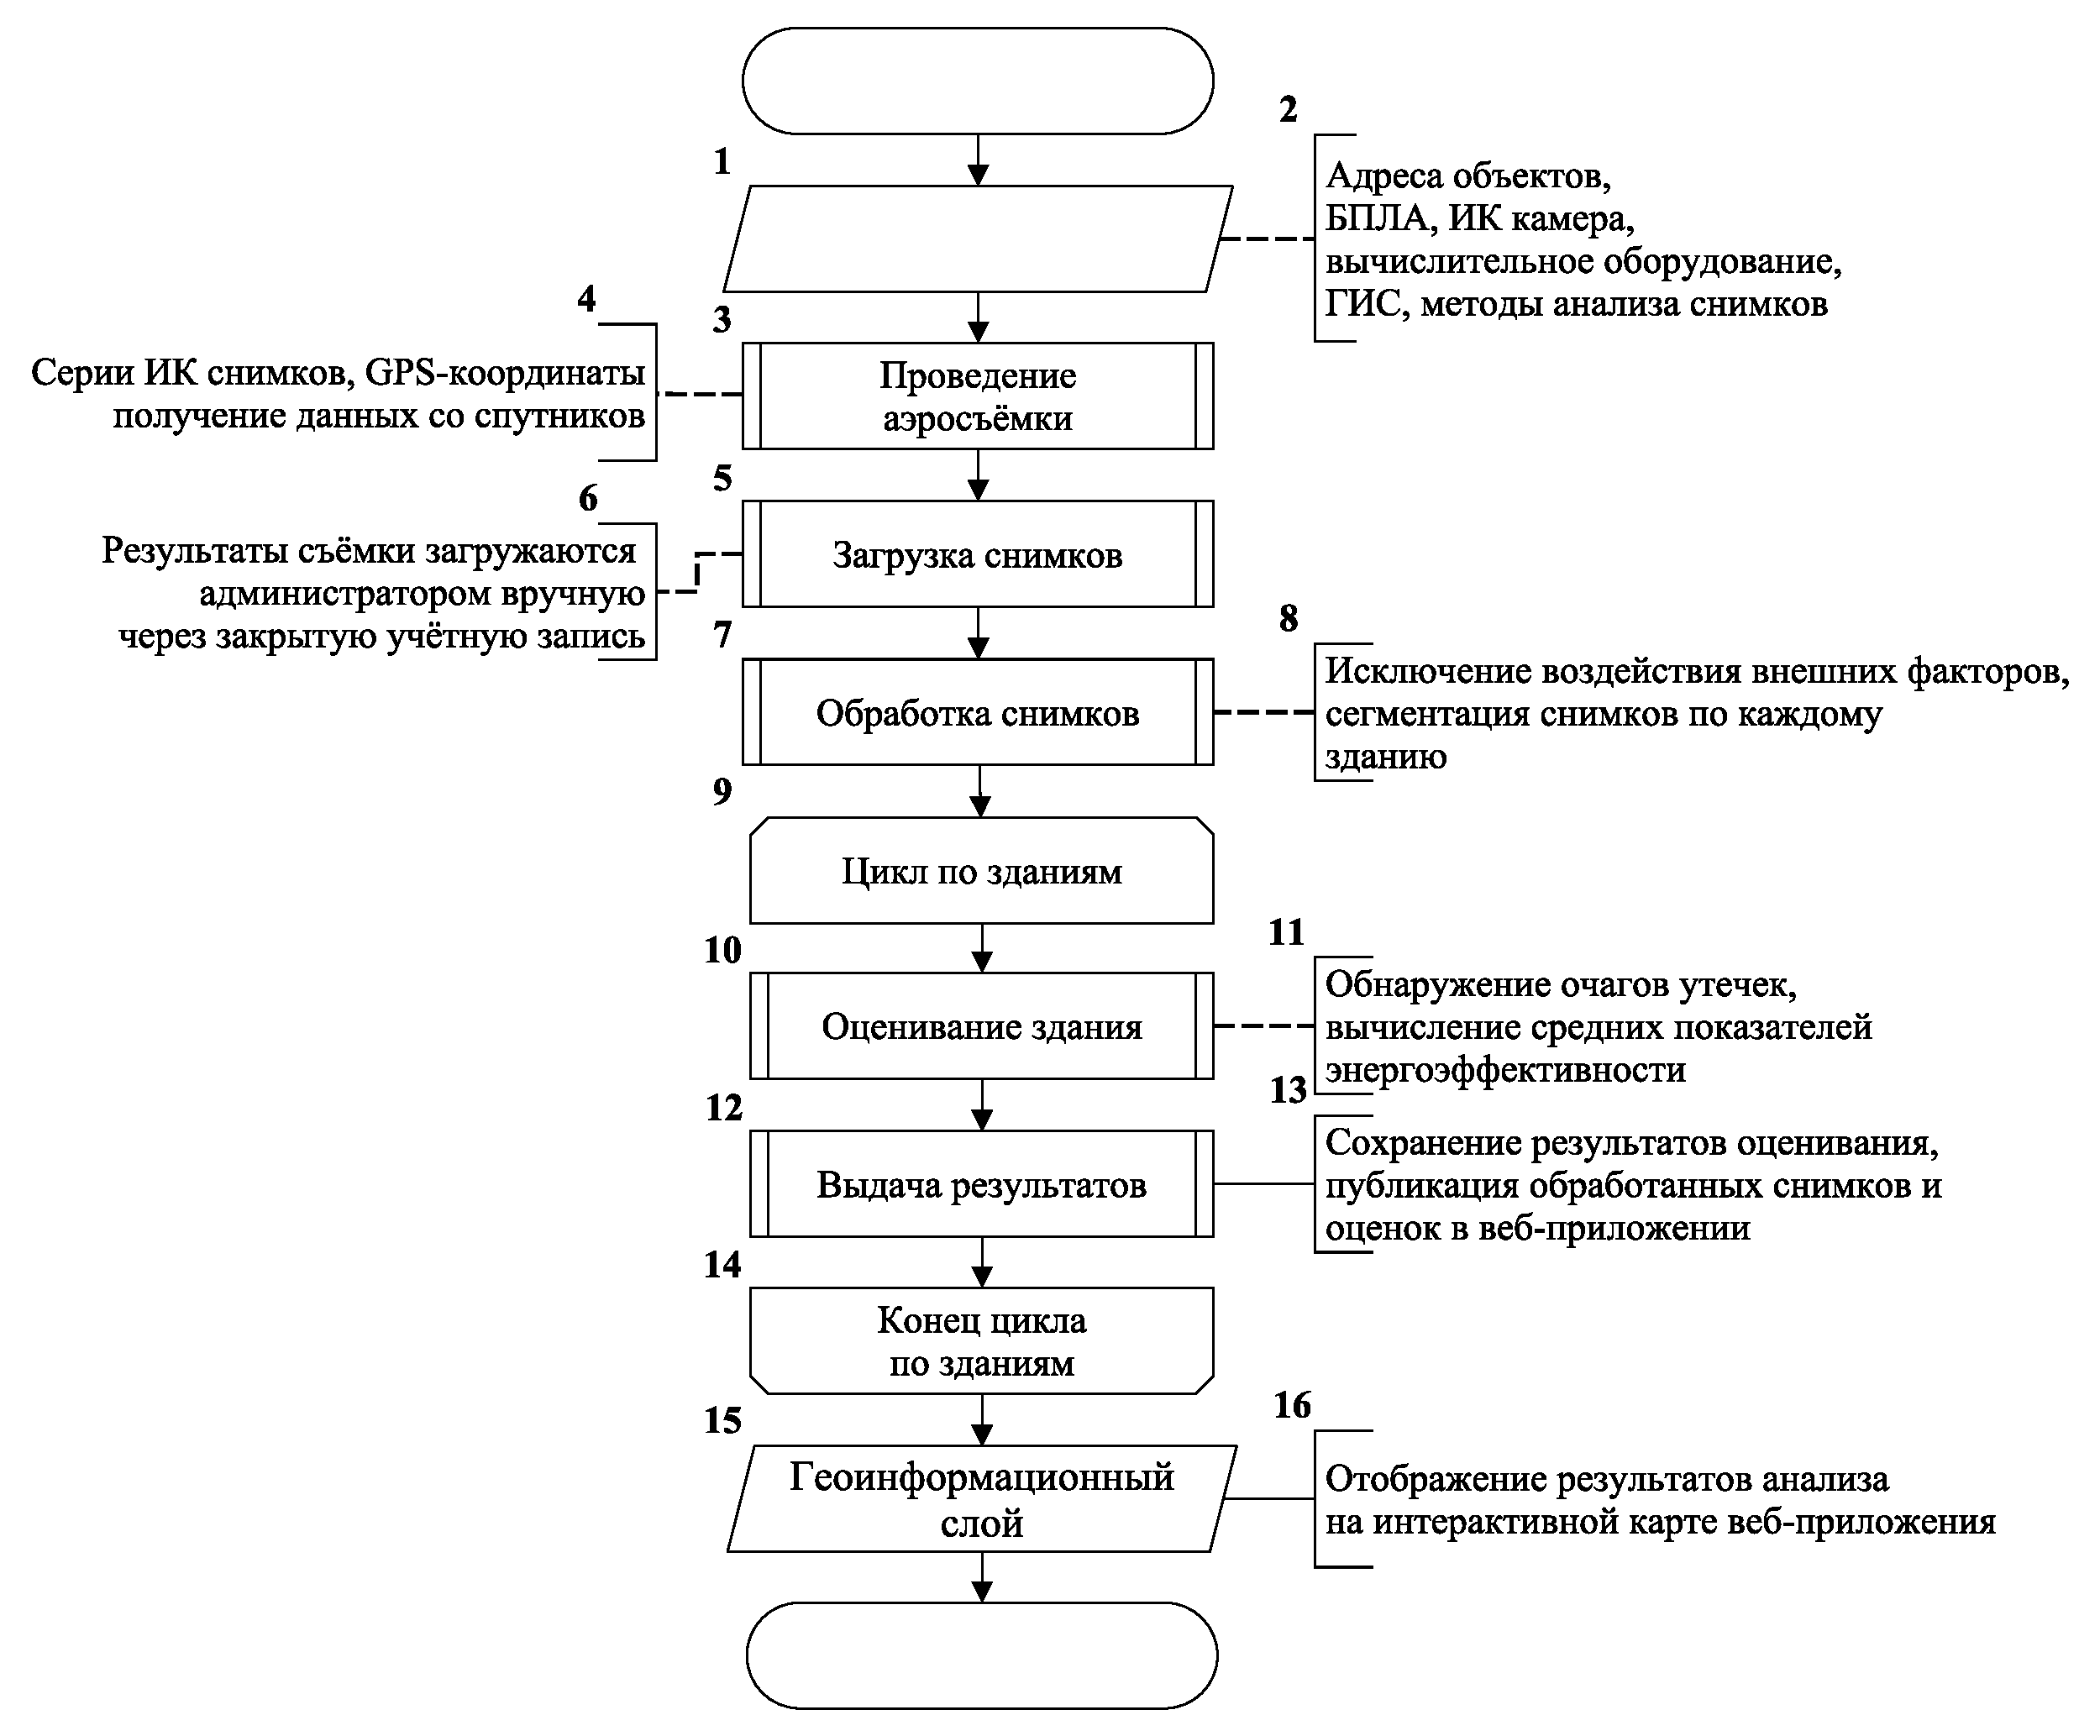
\includegraphics[width=0.9\textwidth]{images/am/am0_before}
      \caption{Алгоритм исследования утечек в жилых зданиях (для прототипа)}
      \label{am:before:common}
    \end{figure}

\pagebreak

	\begin{figure}[h!]
      \centering
      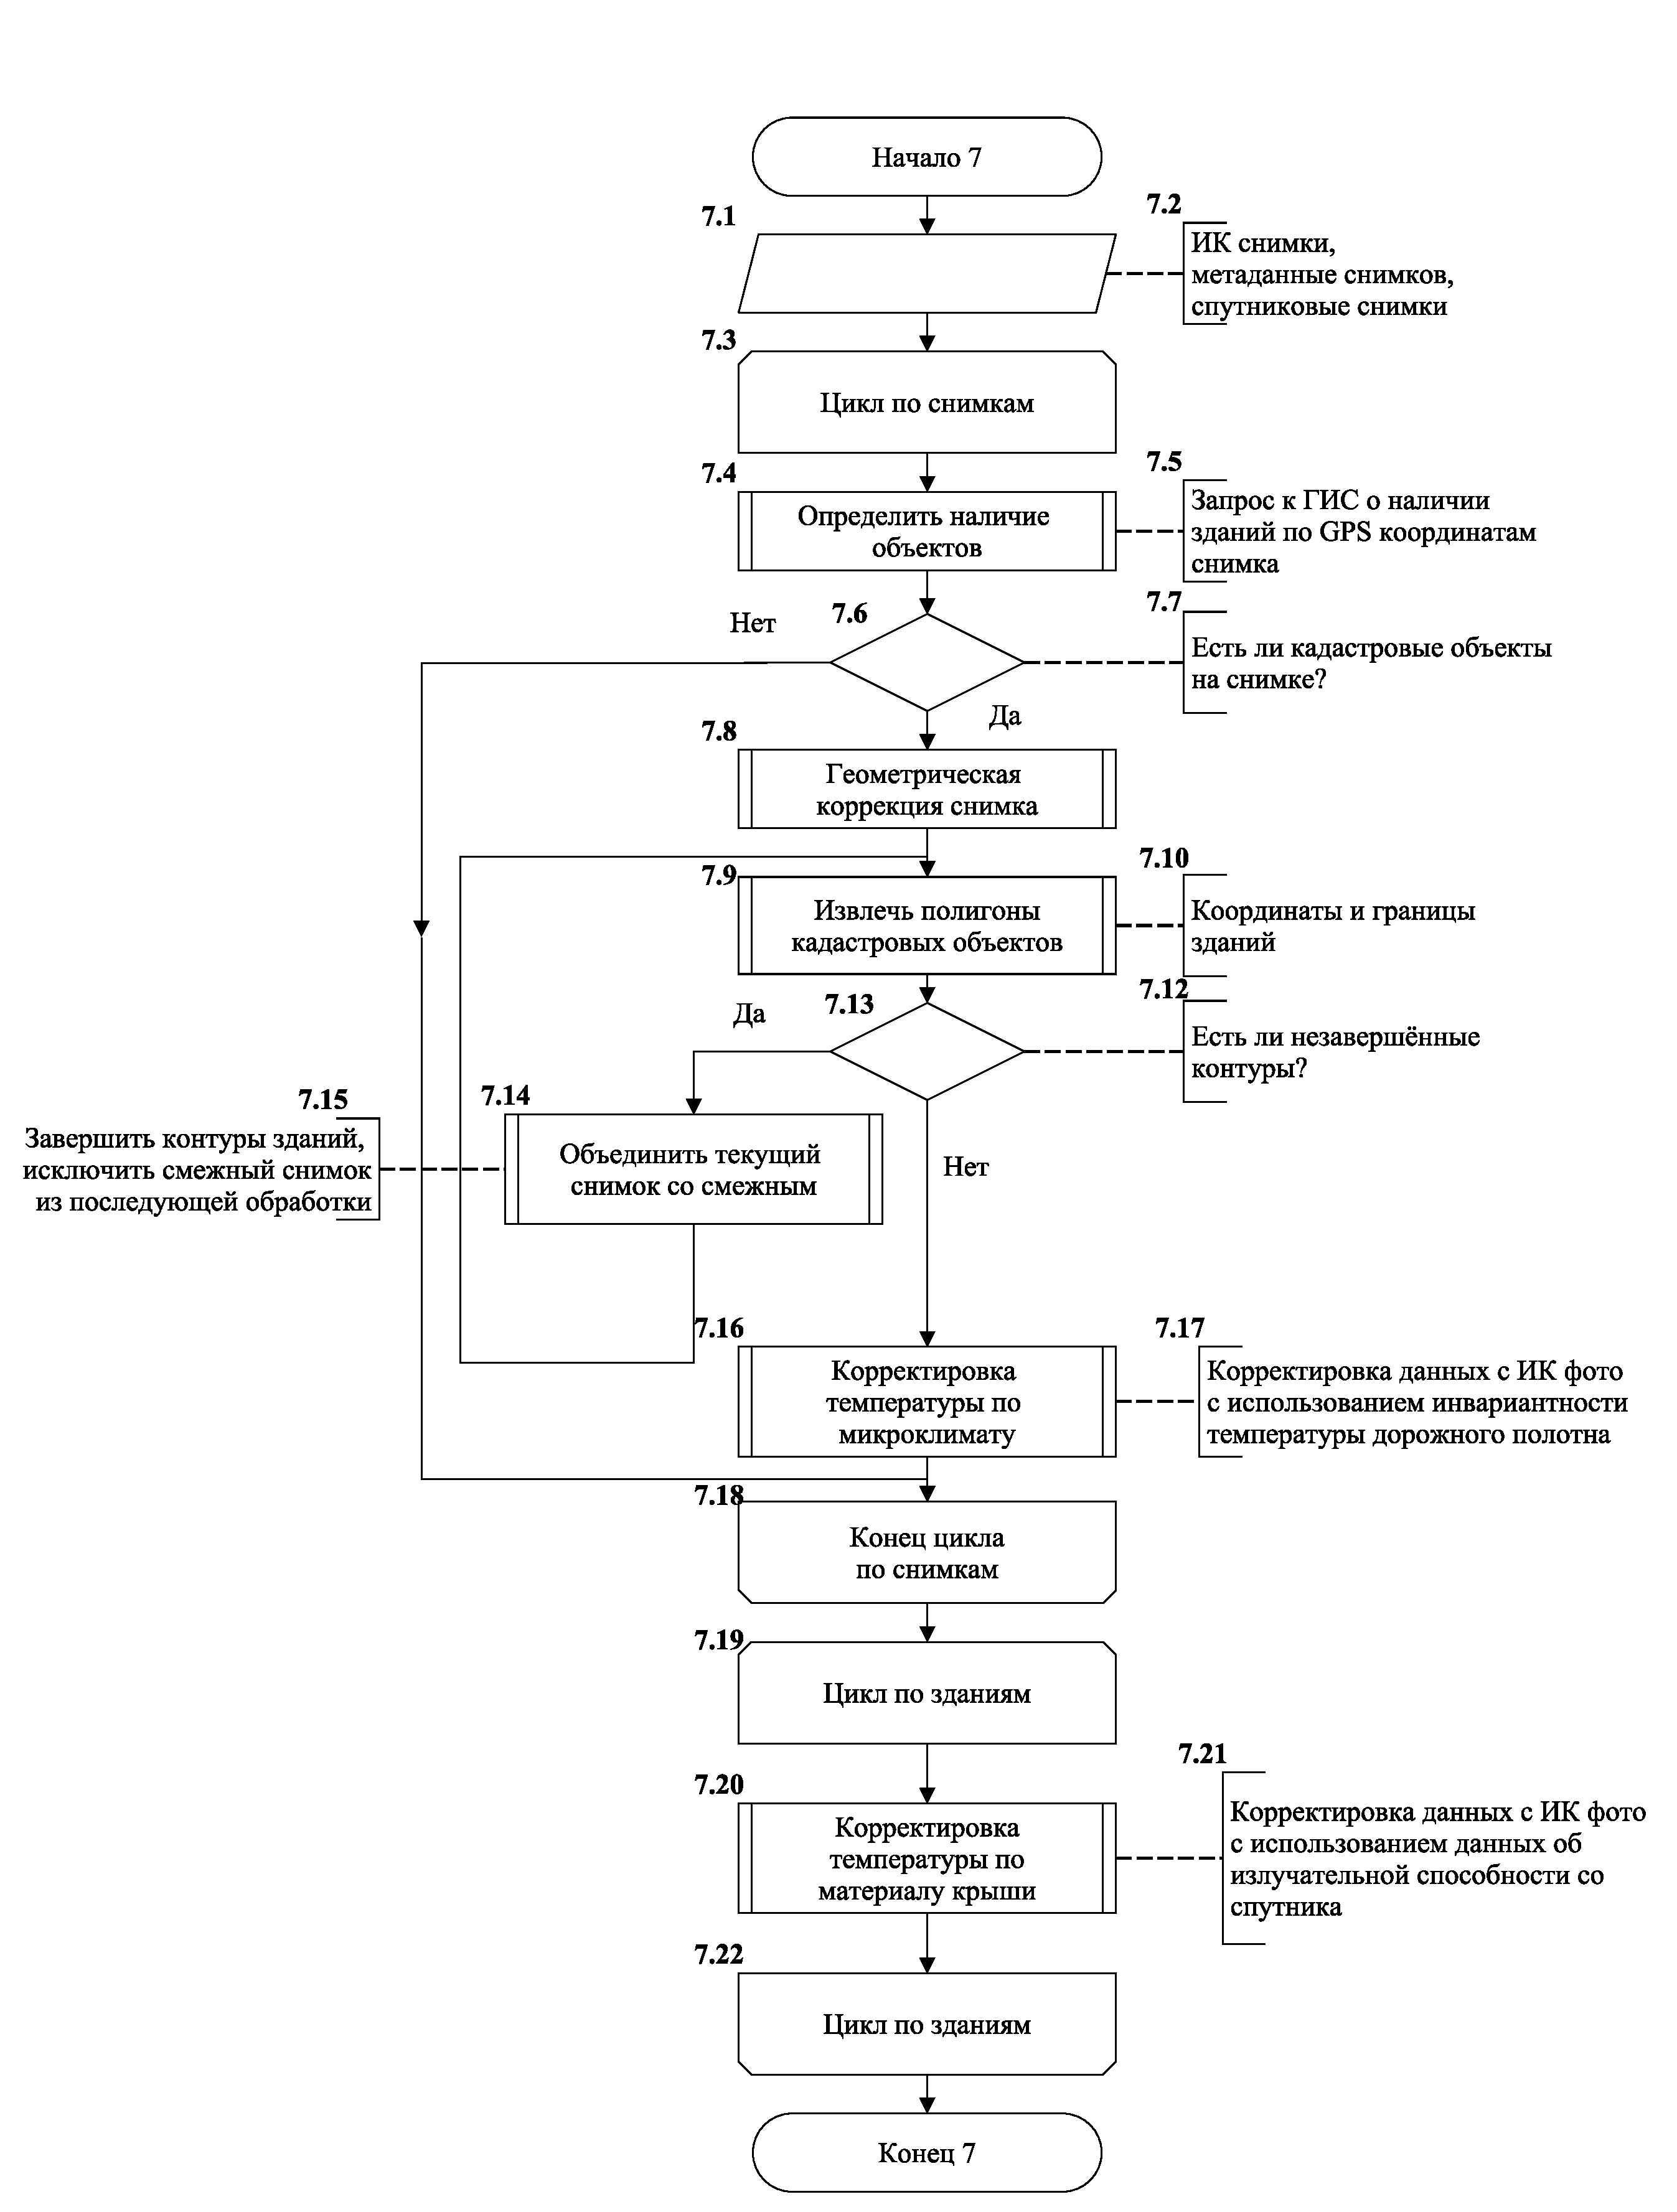
\includegraphics[width=0.9\textwidth]{images/am/am01_before}
      \caption{Алгоритм обработки аэроснимков (для прототипа)}
      \label{am:before:aero}
    \end{figure}    



\subsection{Алгоритмическая модель предлагаемого решения}
\label{sec:models:algo:after}

\par
	В связи с тем, что предлагаемая система предполагает два вида съёмки, изменяется основной алгоритм исследования утечек жилых зданий для расчёта оценки их энергоэффективности (рисунок \ref{am:after:common}). Возникает проблема, связанная с тем, что одно здание может быть отснято несколько раз, причём разным способом. Для решения этой проблемы следует проводить интегральную (итоговую) оценку, представленную в алгоритме процессом 20. Более детальное описание этого процесса описывает алгоритм, приведённый на рисунке 
	\ref{am:after:integral}.

	\begin{figure}[h!]
      \centering
      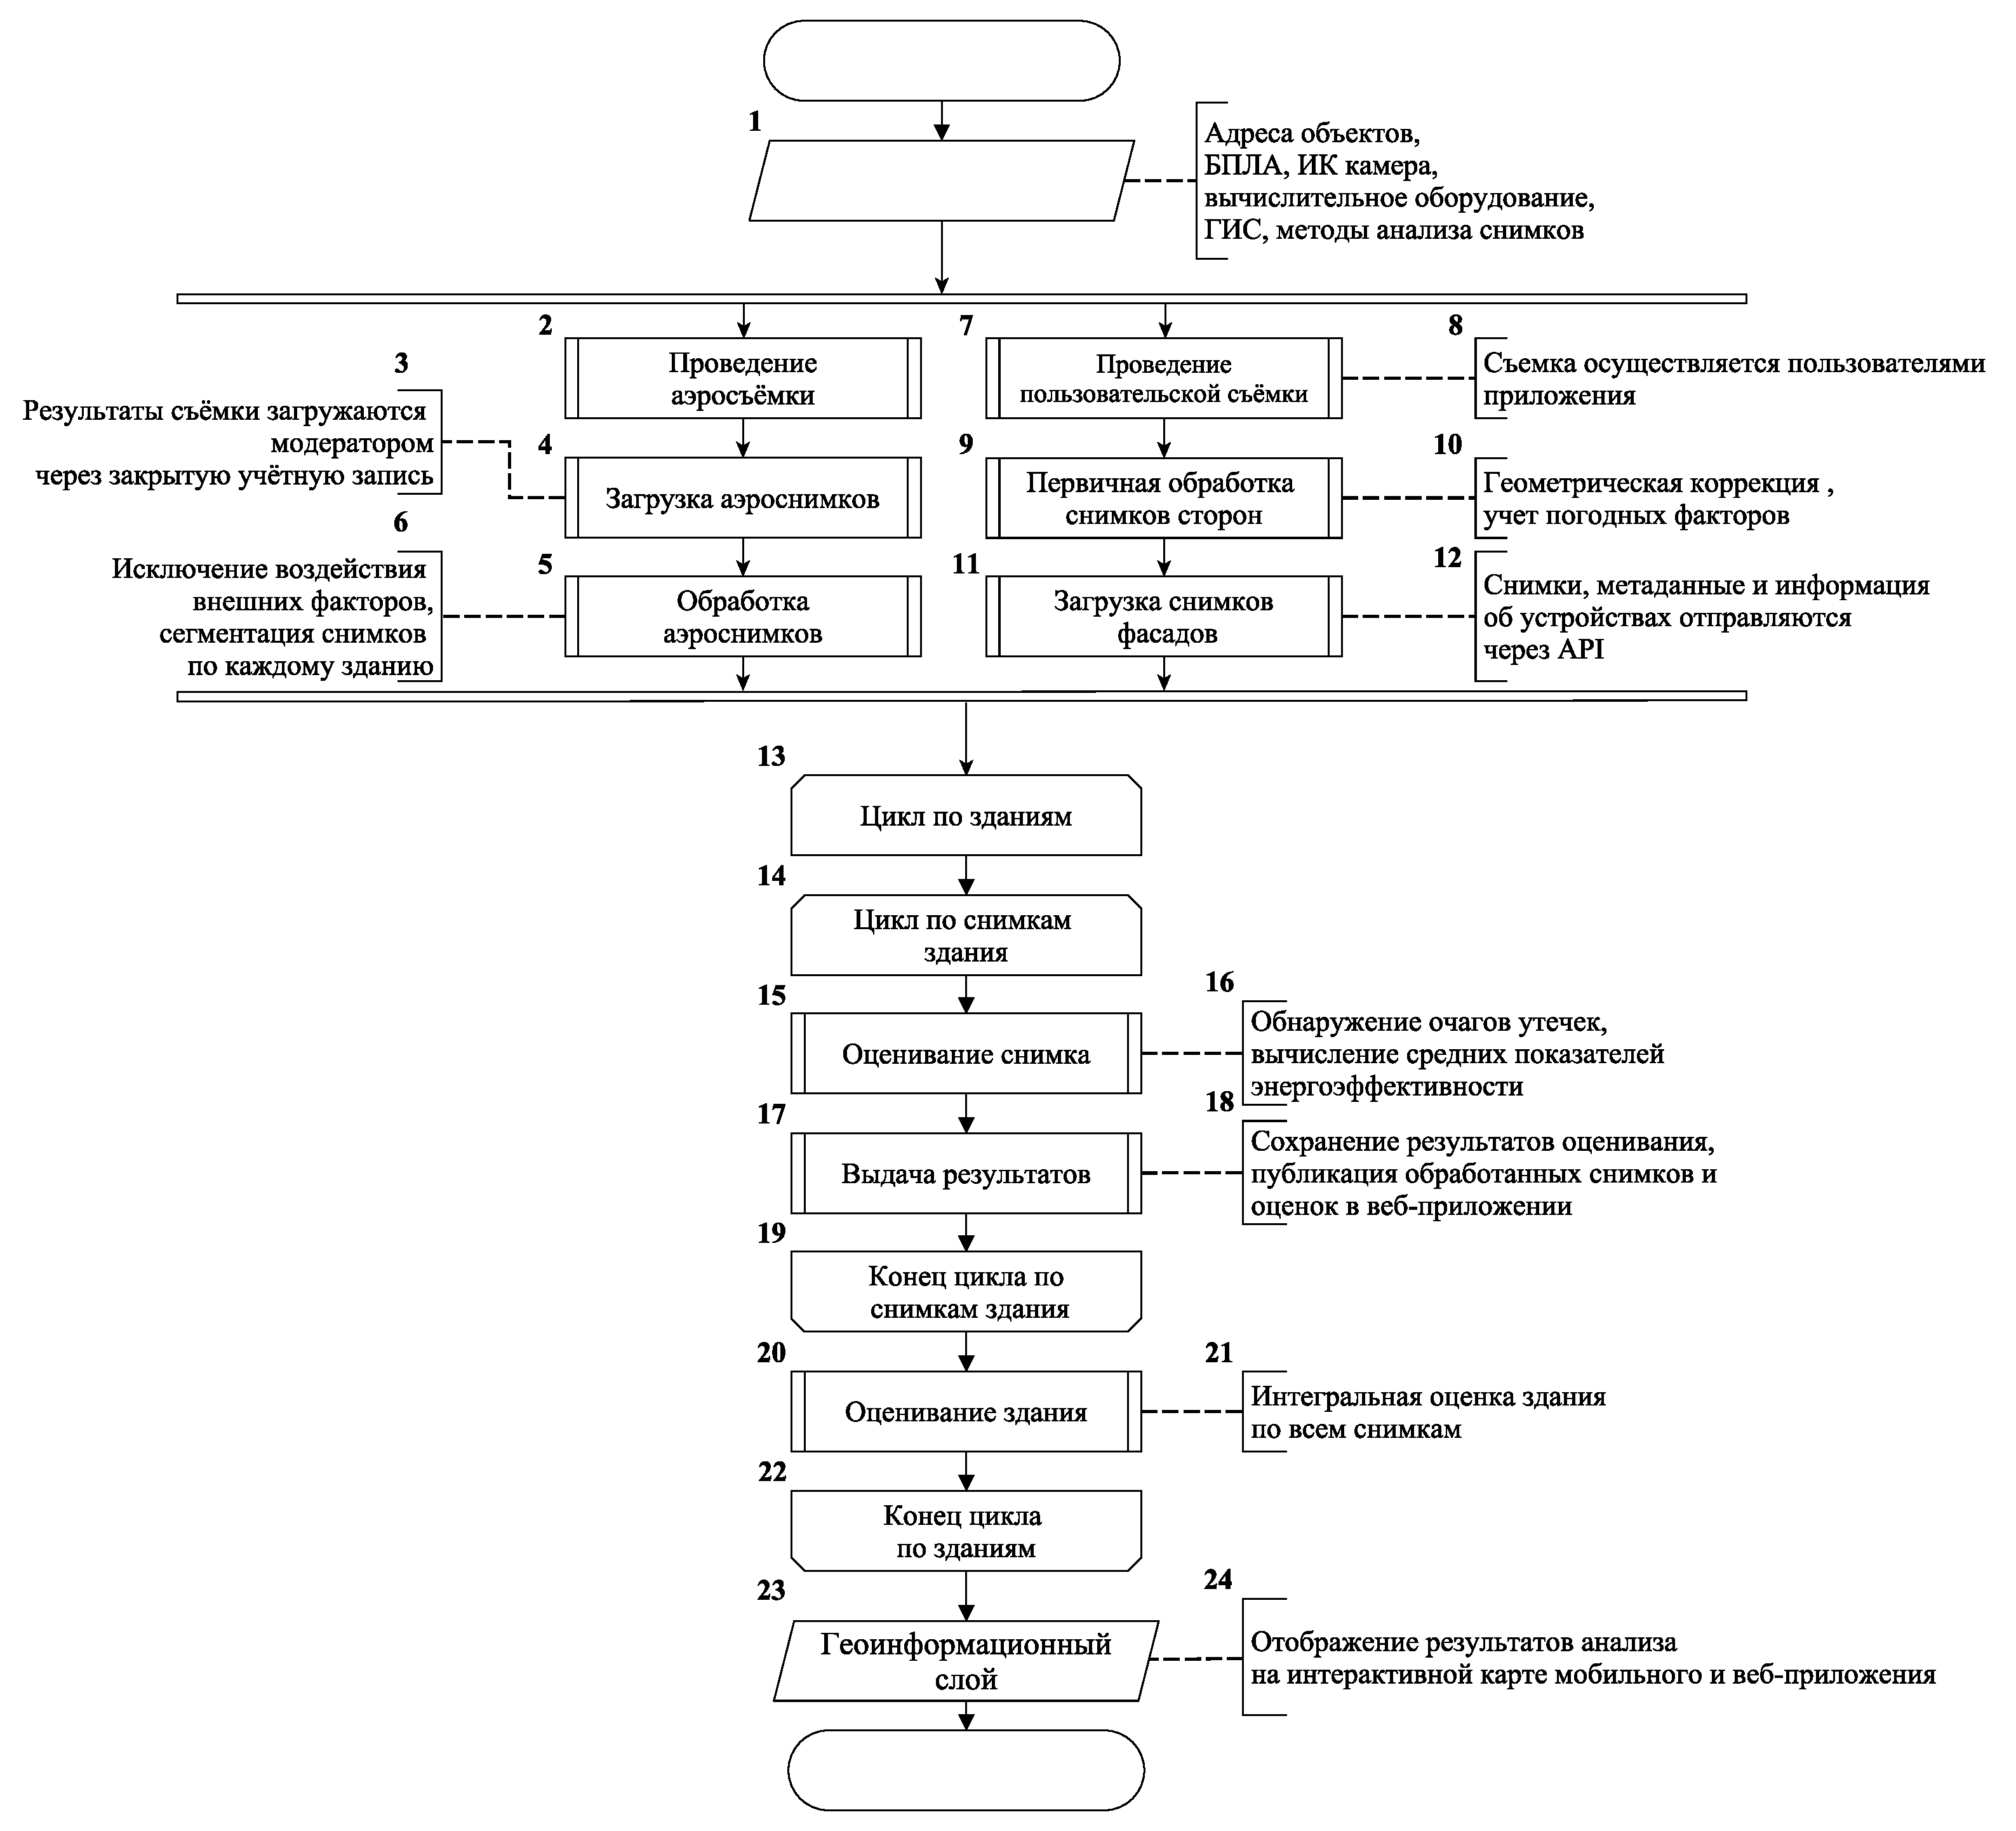
\includegraphics[width=0.9\textwidth]{images/am/am0_after}
      \caption{Алгоритм исследования утечек в жилых зданиях (для предлагаемого решения)}
      \label{am:after:common}
    \end{figure}

    \begin{figure}[t!]
      \centering
      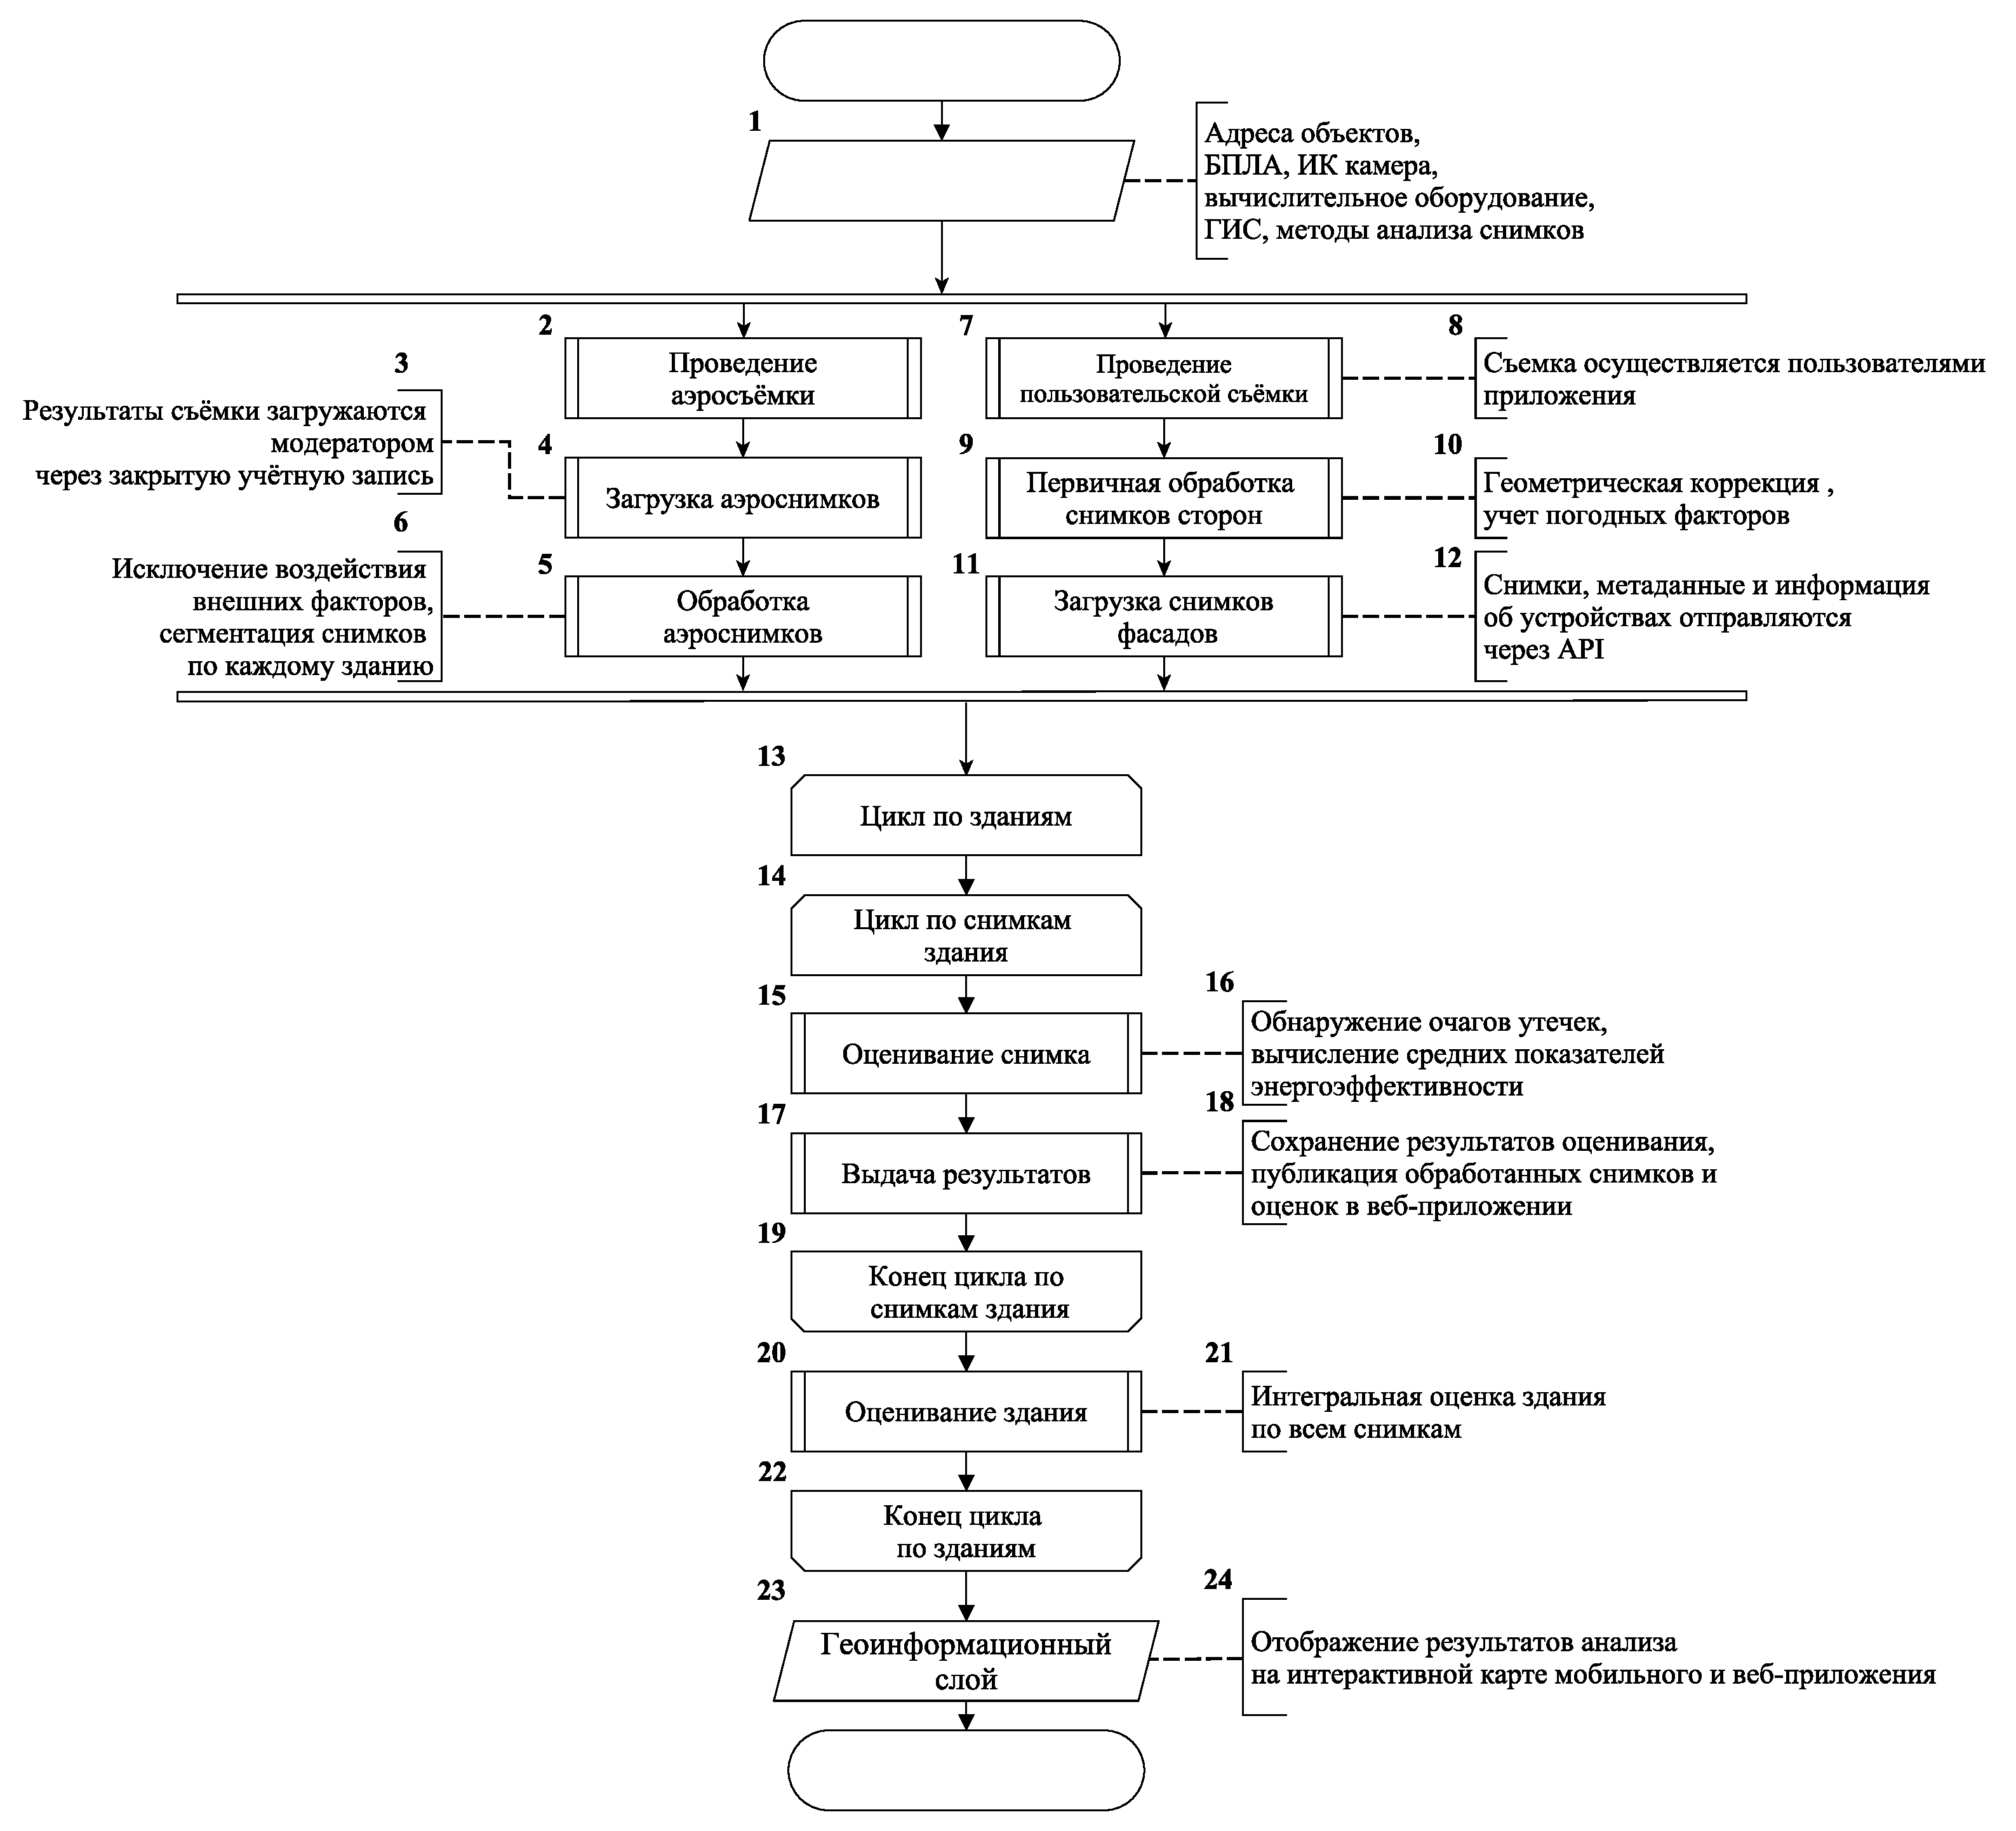
\includegraphics[width=0.9\textwidth]{images/am/am0_after}
      \caption{Алгоритм итогового оценивания энергоэффективности (для предлагаемого решения)}
      \label{am:after:integral}
    \end{figure}

\pagebreak

\par
	После внедрения новых подсистем процедура получения пользователем информации из системы также претерпевает изменения. Сравнение алгоритмов работы с системой до изменений (рисунок \ref{am:before:common}) и после них (рисунок \ref{am:after:common}) позволяет их выделить.

	\begin{figure}[t!]
      \centering
      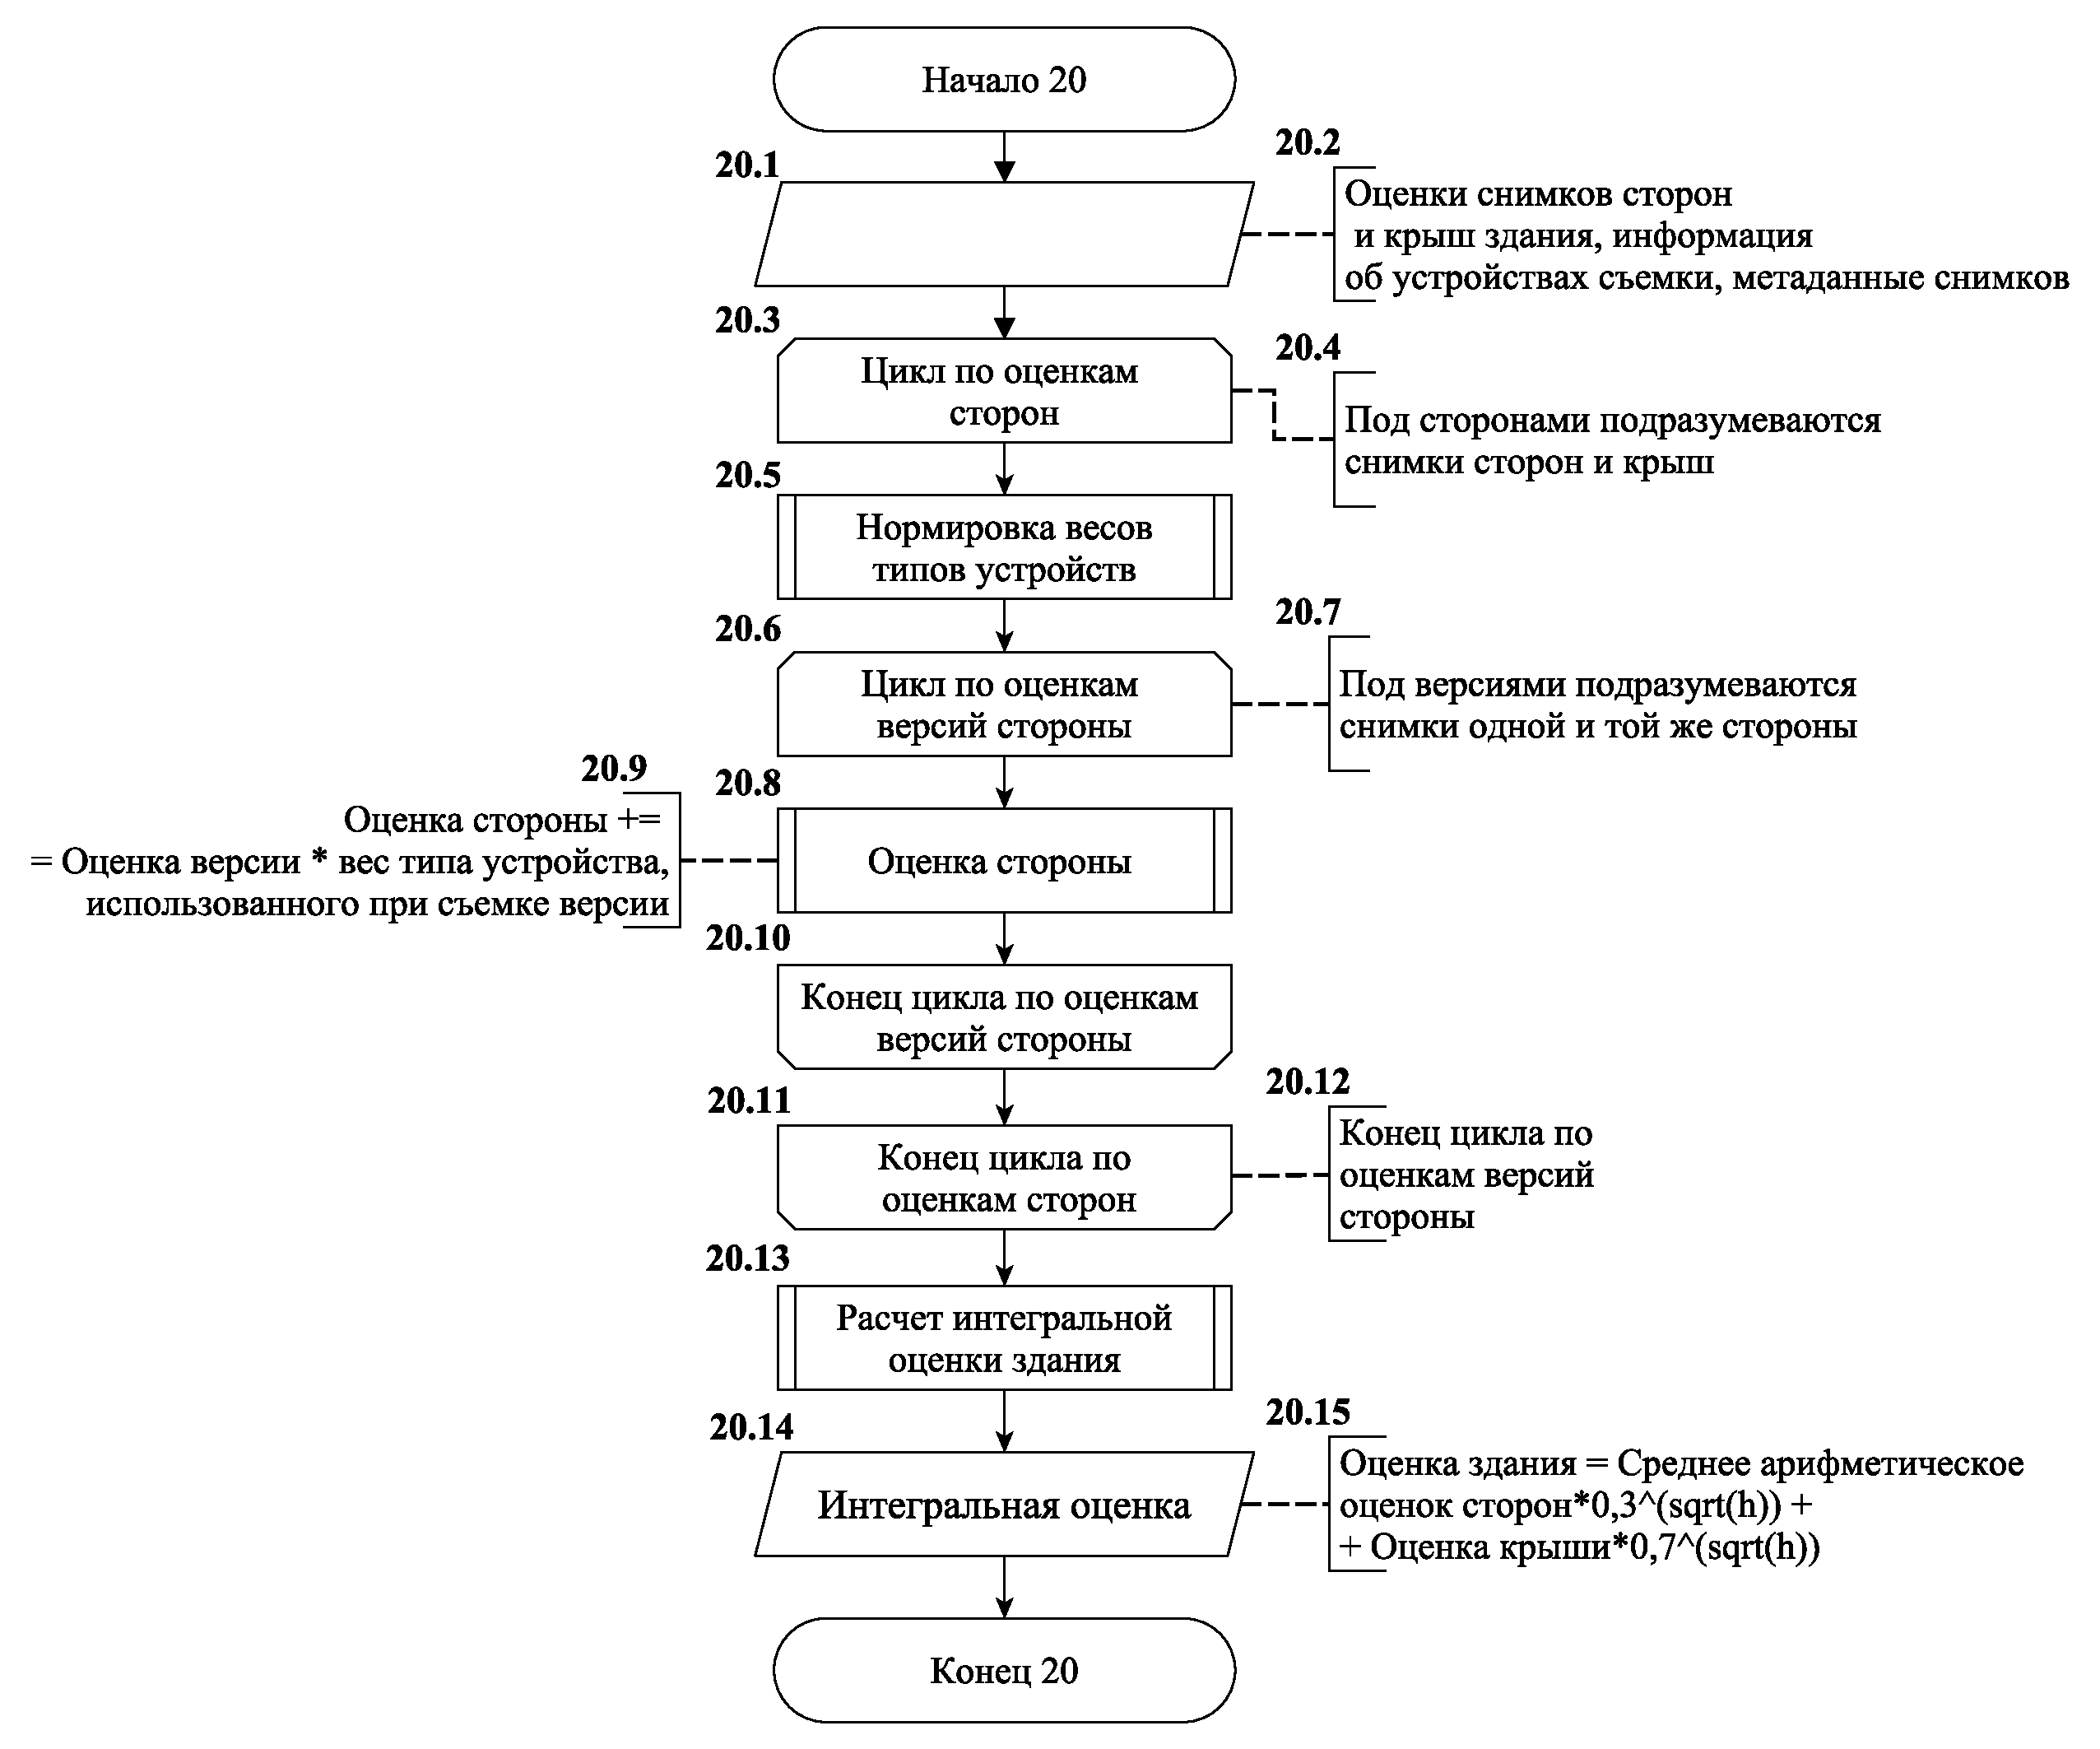
\includegraphics[width=0.9\textwidth]{images/am/am02_after}
      \caption{Алгоритм итогового оценивания энергоэффективности (для предлагаемого решения)}
      \label{am:after:common}
    \end{figure}

\pagebreak

\subsection{Результаты и выводы по главе 2}
\label{sec:models:summary}

\par
	На основе информации, полученных в результате изучения материалов, приведённых в главе 1, были построены модели прототипа и предлагаемого решения. В целях выделения специфики между существующей системой и предлагаемым решением представлена структурно-функциональная модель и алгоритмы работы с подсистемами прототипа и новой системы.

	Благодаря тому, что моделирование проводилось как для системы в целом, так и для разрабатываемого программного интерфейса (API), можно получить представление о том, как изменяются отдельные компоненты системы, как взаимодействуют информационные потоки смежных с API подсистем и внешней среды всей системы анализа тепловых утечек. Взаимосвязь между системой в целом и её подсистемами показана в концептуальной, системно-структурной и структурно-функциональной моделях.

	Алгоритмы, представленные в разделе \ref{sec:models:algo}, имеют целью продемонстрировать ключевые изменения в работе компонентов системы, а также в работе пользователей с системой. Кроме того, смоделирован алгоритм работы разрабатываемого API, который отражает специфику на фоне аналогов в области разработки программных интерфейсов.

	Таким образом, становится возможным формулирование конкретного списка требований, которым должны удовлетворять все подсистемы в новом решении на этапе проектирования и задач, которые необходимо выполнить при реализации нового решения в рамках данной работы.
